\section*{Problem 12 - Linear and decision-feedback MIMO detection}
\begin{align*}
	& \text{\uline{MIMO-MRC}} \\
	& \sigma_{n_1}^2=\sigma_{n_2}^2=\ldots=\sigma_{N_R}^2=\sigma_n^2 \\
	& 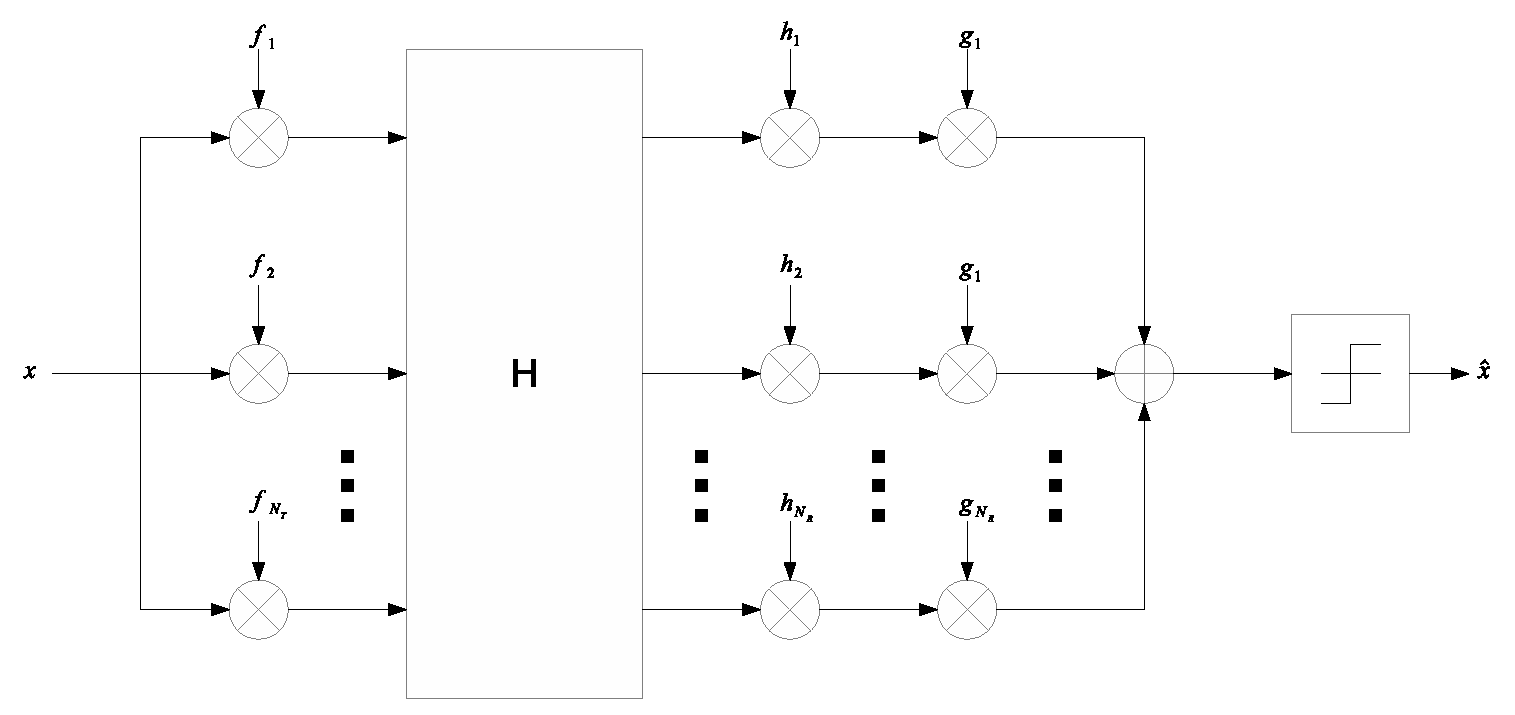
\includegraphics[width=1\textwidth]{MIMO_MRC.eps} \\
	& f=\left(f_1,f_2,\ldots,f_{N_R}\right)^T;\qquad g=\left(g_1^*,g_2^*,\ldots,g_{N_R}^*\right) \\
	& \quad\rightarrow\quad\text{Nomenclature:}\quad
	\begin{cases}
	f^Hf=1=\|f\|^2 \\
	g^Hg=1=\|g\|^2
	\end{cases} \\
	& \text{singular value decomposition:}\quad\mathbf{H=U\Sigma V}^H \\
	& \mathbf{\Sigma} =\diag\left(\xi_1^2,\xi_2^2,\ldots,\xi_N^2\right) \\
	& \quad\rightarrow\quad\text{sorted in descending order}\quad\rightarrow\quad\xi_1^2=\xi_{max}^2 \\
	& f = \mathbf{V}f'\quad\rightarrow\quad\mathbf{V}^Hf=\underbrace{\mathbf{V}^H\mathbf{V}}_{\mathbf{I}}f'=f'\quad\rightarrow\quad\|f'\|^2=\|\mathbf{V}^Hf\|^2\overset{\mathbf{V}: unitary}{=}\|f\|^2=1 \\
	& \text{in a similar way:} \\
	& \quad\rightarrow\quad g=u\cdot g' \\
	& \quad\rightarrow\quad \|g\|^2=\|g'\|^2=1 \\
	& \mathrm{SNR}=\frac{\sigma_x^2\left|\overbrace{h_{total}}^{\substack{\text{total transfer} \\ \text{function}}}\right|^2}{\sigma_n^2\underbrace{\|g\|^2}_{\rightarrow =1}}= \frac{\sigma_x^2\left|g^HHf\right|}{\sigma_n^2}=\frac{\sigma_x^2\left|g'^H\mathbf{U}^H\mathbf{U\Sigma V}^H\mathbf{V}f'\right|}{\sigma_n^2} \\
\end{align*}
\begin{align*}
	& \quad\rightarrow\quad\mathrm{SNR}=\frac{\sigma_x^2}{\sigma_n^2}\left|g'^H\mathbf{\Sigma}f'\right| \\
	& g'=\begin{pmatrix}1&0&\ldots&0\end{pmatrix}';\quad f'=\begin{pmatrix}1&0&\ldots&0\end{pmatrix}' \\
	& \quad\rightarrow\quad\text{to maximize SNR: }\xi_1=\xi_{max} \\
	& \quad\quad\quad\mathrm{SNR_{max}}=\frac{\sigma_x^2}{\sigma_n^2}\xi_1^2 \\
	& \text{$\xi_k^2$ are also eigenvalues of $HH^H$} \\
	& \quad\|H\|_F^2=\tr\left(HH^H\right)=\sum\limits_{k=1}^N\xi_k^2\qquad N=\min\{N_T,N_R\} \\
	& \text{Frobenius norm} \\
	& \xi_1^2=\xi_{max}^2\quad\rightarrow\quad\underbrace{\frac{1}{N}\sum\limits_{k=1}^N\xi_k^2}_{\text{average}}\le\xi_{max}^2\le\sum\limits_{k=1}^N\xi_k^2 \\
	& \|H\|_F^2=\sum\limits_{i=1}^{N_T}\sum\limits_{j=1}^{N_R}\left|h_{ij}\right|^2,\quad h_{ij}\sim C\mathcal{N}\left(0,1\right) \\
	& \quad\rightarrow\quad\|H\|_F^2\text{ is the sum of squared complex Gaussian RVs} \\
	& \quad\rightarrow\quad\text{$\chi^2$-square ($\chi^2$-distribution} \\
	& f_{{\|H\|}_F^2}\left(x\right)=\frac{1}{\Gamma\left(N_TN_R\right)}x^{N_TN_R-1}e^{-x} \\
	& \overbrace{f_{\frac{1}{N}{\|H\|}_F^2}}^{\text{pdf of the channel}}=\frac{1}{\Gamma\left(N_TN_R\right)}\left(Nx\right)^{N_TN_R-1}e^{-Nx} = \frac{N^{N_TN_R}x^{N_TN_R-1}e^{-Nx}}{\Gamma\left(N_TN_R\right)} \\
	& \overline{\mathrm{SER}}\ge\int\limits_0^\infty f_{\frac{1}{N}{\|H\|}_F^2}\mathrm{SER}\left(x\right)\mathrm{d}x = \int\limits_0^\infty\frac{N^{N_TN_R}x^{N_TN_R-1}e^{-Nx}}{\Gamma\left(N_TN_R\right)}\frac{C_\mathcal{A}}{2}e^{-\frac{d_\mathcal{A}^2}{2}x\gamma}\mathrm{d}x= \\
	& \qquad=\frac{N^{N_TN_R}C_\mathcal{A}}{2\Gamma\left(N_TN_R\right)}\int\limits_0^\infty x^{N_TN_R-1}e^{-\left(N+\frac{d_\mathcal{A}^2}{2}\gamma\right)x}\mathrm{d}x=\frac{N^{N_TN_R}C_\mathcal{A}}{2\Gamma\left(N_TN_R\right)}\frac{\Gamma\left(N_TN_R\right)}{\left(N+\frac{d_\mathcal{A}^2}{2}\gamma\right)^{N_TN_R}} \\
	& \rightarrow\quad\overline{\mathrm{SER}}\ge\frac{C_\mathcal{A}N^{N_TN_R}}{2\left(N+\frac{d_{\mathcal{A}^2}}{2}\underbrace{\gamma}_{\mathrm{SNR}}\right)^{N_TN_R}} \\
	& \mathrm{SNR}\quad\rightarrow\quad\infty\quad\Rightarrow\quad\mathrm{SER}\ge\frac{C_\mathcal{A}}{2\left(\frac{d_\mathcal{A}^2}{2N}\gamma\right)^{N_TN_R}}
\end{align*}
\begin{align*}
	& \frac{\sum\limits_{k=1}^N\xi_k^2}{N}\le\xi_{max}^2\le\sum\limits_{k=1}^N\xi_k^2\quad\rightarrow\quad\overline{\mathrm{SER}}\le\frac{C_\mathcal{A}}{2\left(\frac{D_\mathcal{A}^2}{2}\gamma\right)^{N_TN_R}} \\
	& \quad\rightarrow\quad\frac{C_\mathcal{A}}{2\left(\frac{D_\mathcal{A}^2}{2N}\gamma\right)^{N_TN_R}}\le\overline{\mathrm{SER}}\le\frac{C_\mathcal{A}}{2\left(\frac{D_\mathcal{A}^2}{2}\gamma\right)^{N_TN_R}} \\
	& \text{we have: }\frac{\ldots}{\ldots\gamma^{N_TN_R}}\quad\rightarrow\quad\text{Diversity gain $=N_TN_R$} \\
\end{align*}
\begin{align*}
	& \text{equalization}
	& \begin{cases}
		\substack{\text{at the receiver}\\ \text{(detection)}} 
			\begin{cases}
				\text{linear} 
					\begin{cases}
						\text{Zero-Forcing ZF} \\
						\text{Minimum Mean Square Error MMSE}
					\end{cases} \\
				\text{decision feedback}
					\begin{cases}
						\text{ZF} \\
						\text{MMSE}
					\end{cases}
			\end{cases} \\
		\substack{\text{at the transmitter}\\ \text{(precoding)}}
			\begin{cases}
				\text{linear} \\
				\text{with feedback}
			\end{cases}
	\end{cases} \\
\end{align*}
\begin{align*}
	& \text{Linear equalizer:} \\
	& 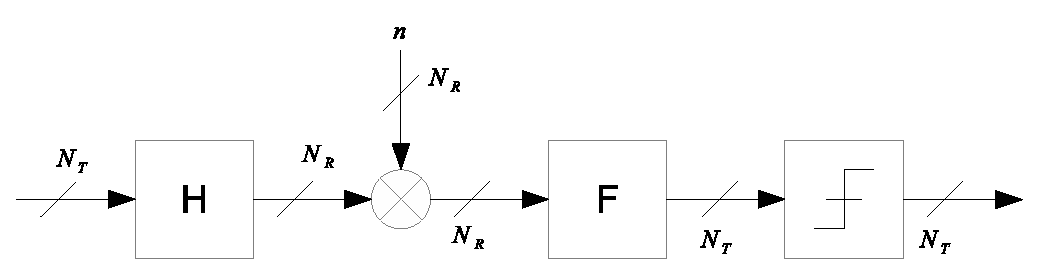
\includegraphics[width=1\textwidth]{linear_equalizer.eps} \\
	& \mathbf{H}\in\mathbb{C}^{N_R\times N_T};\qquad\mathbf{F}\in\mathbb{C}^{N_T\times N_R} \\
	& \mathbf{H}=
	\begin{pmatrix}
	0,2 & -0,2 \\
	0,1 & 0,4 \\
	1 & 0,2
	\end{pmatrix},\qquad\frac{\sigma_x^2}{\sigma_n^2}=10 \\
	& N_R>N_T\quad\rightarrow\quad \mathbf{F}=\left(\mathbf{H}^H\mathbf{H}\right)^{-1}\cdot\mathbf{H}^H\quad\rightarrow\quad\text{left Moore-Penrose pseudo-inverse} \\
	& \text{received signal: }r=\mathbf{FH}x+\mathbf{F}n\quad\rightarrow\quad\text{drawback: noise amplification} \\
	& r=\mathbf{FH}x+\mathbf{F}n=\underbrace{\left(\mathbf{H}^H\mathbf{H}\right)^{-1}\mathbf{H}^H\mathbf{H}}_{\mathbf{I}}x+\mathbf{F}n=x+\mathbf{F}n\quad\rightarrow\quad\text{no interference} \\
	& \rightarrow\quad\text{error signal: }e=\mathbf{F}n\quad\rightarrow\quad\phi_{ee}=ee^H=\mathbf{F}\underbrace{nn^H}_{\sigma_n^2\mathbf{I}}\mathbf{F}^H \\
	& \qquad\rightarrow\quad nn^H=\sigma_n^2\mathbf{I}\quad\text{white noise}
\end{align*}
\begin{align*}
	& \rightarrow\quad\phi_{ee}^{ZF}=\sigma_n^2\mathbf{FF}^H\quad\rightarrow\quad\phi_{ee}^{ZF}=\sigma_n^2
	\begin{pmatrix}
	1,13 & -0,94 \\
	-0,94 & 4,95
	\end{pmatrix} \\
	& \sigma_e^2=\tr\left(\phi_{ee}^{ZF}\right)=\sigma_n^2\left(1,13+4,95\right) \\
	& \Rightarrow\sigma_e^2=\sigma_n^2\cdot 6,1 \\
	& \text{Now determine $\mathbf{F}$ such that the error-variance is minimal!} \\
	& \rightarrow\quad\text{MMSE}\quad\rightarrow\quad\mathbf{F}=\left(\mathbf{H}^H\mathbf{H}+\frac{\sigma_n^2}{\sigma_x^2}\mathbf{I}\right)^{-1}\underbrace{\mathbf{H}^H}_{\substack{\text{matched}\\ \text{filter}}};\qquad\frac{\sigma_x^2}{\sigma_n^2}=10 \\
	& \Rightarrow\text{for low SNR: MMSE} \\
	& \Rightarrow\text{for high SNR: ZF} \\
	& \rightarrow\mathbf{F}=
	\begin{pmatrix}
	0,31 & -0,13 & 0,85 \\
	-0,77 & 1,25 & 0,086
	\end{pmatrix} \\
	& \rightarrow\text{from lecture notes:} \\
	& \quad\rightarrow\quad\phi_{ee}=\sigma_n^2\left(\mathbf{H}^H\mathbf{H}+\frac{\sigma_n^2}{\sigma_x^2}\mathbf{I}\right)^{-1}\quad\rightarrow\quad\phi_{ee}^{MMSE}=\sigma_n^2
	\begin{pmatrix}
	0,97 & -0,57 \\
	-6,57 & 3,28
	\end{pmatrix} \\
	& \quad\rightarrow\quad\text{total error variance = }\tr\left(\phi_{ee}\right) \\
	& \qquad\Rightarrow\quad\sigma_e^2=4,25\sigma_n^2 \\
	& \text{End-to-end channel: }\mathbf{K=FH=}
	\begin{pmatrix}
	0,9 & 0,06 \\
	0,06 & 0,67
	\end{pmatrix} \\
	& \text{residual interference in off-diagonal elements} \\
	&	\text{diagonal elements should be 1, but are not $\Rightarrow$ biased!} \\
	& \rightarrow\text{solution:}\quad\rightarrow\quad\text{remove bias by multiplying with }\mathbf{C}=
	\begin{pmatrix}
	\frac{1}{0,9} & 0 \\
	0 & \frac{1}{0,67}
	\end{pmatrix} \\
	& \rightarrow\mathbf{C}=
	\begin{pmatrix}
	1,11 & 0 \\
	0 & 1,49
	\end{pmatrix} \\
	& r'=\mathbf{C}r=
	\begin{pmatrix}
	1,11 & 0 \\
	0 & 1,49
	\end{pmatrix}
	\begin{pmatrix}
	0,9 & 0,06 \\
	0,06 & 0,67
	\end{pmatrix}x+
	\begin{pmatrix}
	1,11 & 0 \\
	0 & 1,49
	\end{pmatrix}\mathbf{F}n=\\
	& =
	\begin{pmatrix}
	1 & 0,07 \\
	0,09 & 1
	\end{pmatrix}x+
	\begin{pmatrix}
	1,11 & 0 \\
	0 & 1,49
	\end{pmatrix}\mathbf{F}n \\
	& \text{from lecture notes:} \\
	& \qquad\phi_{e'e'}=\sigma_x^2\left(\mathbf{I}+\left(\mathbf{C-I}\right)\mathbf{K}^H\mathbf{C}^H-\mathbf{CK}\right);\qquad\frac{\sigma_x^2}{\sigma_n^2}=10 \\
	& \qquad\Rightarrow\quad\sigma_x^2
	\begin{pmatrix}
	0,11 & -0,05 \\
	-0,05 & 0,49
	\end{pmatrix}=\sigma_n^2
	\begin{pmatrix}
	1,1 & -0,5 \\
	-0,5 & 4,5
	\end{pmatrix} \\
	& \qquad\rightarrow\quad\sigma_e'^2=\tr\left(\phi_{e'e'}\right)=6\sigma_n^2
\end{align*}
\begin{align*}
	& \text{Decision feedback:} \\
	& 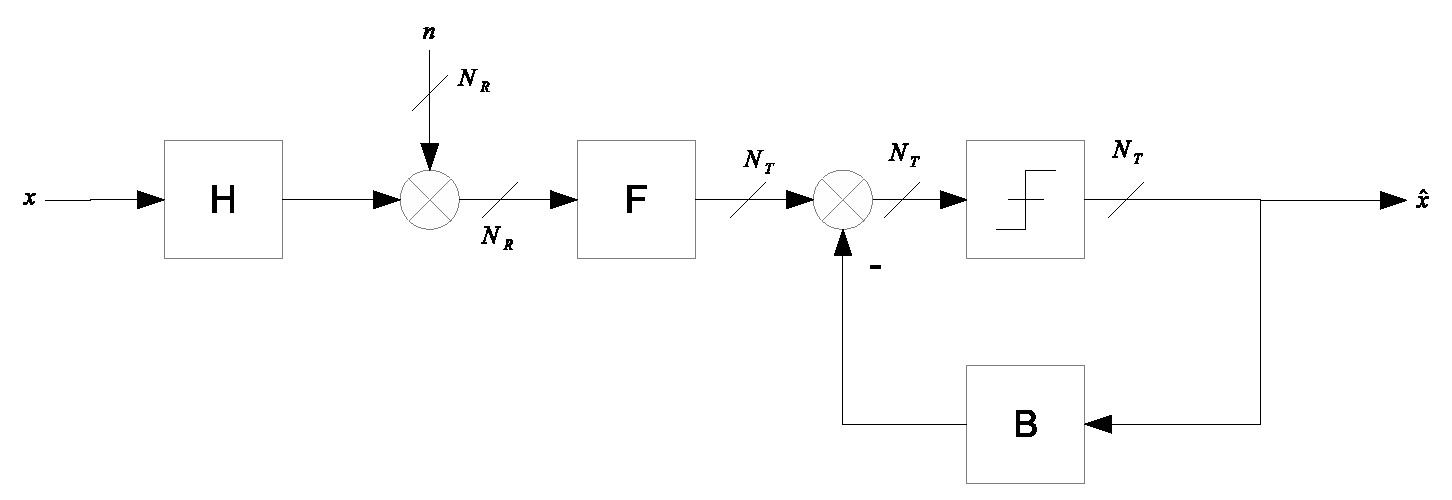
\includegraphics[width=1\textwidth]{decisionfeedback_equalizer.eps} \\
	& \mathbf{H}\in\mathbb{C}^{N_R\times N_T};\qquad\mathbf{F}\in\mathbb{C}^{N_T\times N_R} \\
	& \text{drawback: propagation of error when errors predictions are not accurate} \\
	& \left[\mathbf{L,D}\right]=???\left(\mathbf{H}^H\mathbf{H}\right)\quad\text{Cholesky factorization} \\
	& \mathbf{H}^H\mathbf{H}=
	\begin{pmatrix}
		1,03 & 0,2 \\
		0,2 & 0,24
	\end{pmatrix}\quad\rightarrow\quad\mathbf{L}=
	\begin{pmatrix}
	1 & 0 \\
	0,19 & 1
	\end{pmatrix},\qquad\mathbf{D}=
	\begin{pmatrix}
	1,03 & 0 \\
	0 & 0,2
	\end{pmatrix} \\
	& \qquad\text{feedforward filter:}\quad\mathbf{F=D}^{-1}\mathbf{C}^{-H}\mathbf{H}^H=
	\begin{pmatrix}
	0,23 & 0,02 & 0,96 \\
	-0,99 & 1,98 & 0,99
	\end{pmatrix} \\
	& \qquad\text{feedback filter:}\quad\mathbf{B=C-I}=
	\begin{pmatrix}
	1 & 0 \\
	0,19 & 1
	\end{pmatrix}-
	\begin{pmatrix}
	1 & 0 \\
	0 & 1
	\end{pmatrix}=
	\begin{pmatrix}
	0 & 0 \\
	0,19 & 0
	\end{pmatrix}
\end{align*}
\begin{align*}
	& \text{MMSE-DFE:} \\
	& \mathbf{LDL}^H=\mathbf{H}^H\mathbf{H}+\frac{\sigma_n^2}{\sigma_x^2}\mathbf{I}=
	\begin{pmatrix}
	1,15 & 0,2 \\
	0,2 & 0,34
	\end{pmatrix}
	\quad\rightarrow\quad\left(\mathbf{L,D}\right)\rightarrow \left(\mathbf{H}^H+\frac{\sigma_n^2}{\sigma_x^2}\mathbf{I}\right) \\
	& \rightarrow\quad\mathbf{L}=
	\begin{pmatrix}
	1 & 0 \\
	0,17 & 1
	\end{pmatrix},\quad\mathbf{D}=
	\begin{pmatrix}
	1,15 & 0 \\
	0 & 0,31
	\end{pmatrix} \\
	& \rightarrow\text{Feedforward filter: }\mathbf{F=C}\left|\mathbf{H}^H\mathbf{H}+\frac{\sigma_n^2}{\sigma_x^2}\mathbf{I}\right|^{-1}\mathbf{H}^H=
	\begin{pmatrix}
	0,19 & 0,21 & 1,13 \\
	0,005 & 0,15 & 0,48
	\end{pmatrix} \\
	& \rightarrow\text{Feedback filter: }\mathbf{B=L-I}=
	\begin{pmatrix}
	0 & 0 \\
	0,1739 & 0
	\end{pmatrix} \\
	& \rightarrow\text{Error covariance matrix: }\phi_{ee}=\sigma_n^2\mathbf{D}^{-1}=\sigma_n^2
	\begin{pmatrix}
	0,87 & 0 \\
	0 & 3,28
	\end{pmatrix} \\
	& \rightarrow\quad\sigma_e^2=\tr\left(\phi_{ee}\right)=4,15\sigma_n^2
\end{align*}